% This is LLNCS.DEM the demonstration file of
% the LaTeX macro package from Springer-Verlag
% for Lecture Notes in Computer Science,
% version 2.4 for LaTeX2e as of 16. April 2010
%
\documentclass{llncs}
%
\usepackage{makeidx}  % allows for indexgeneration
\usepackage{graphicx}
%
\begin{document}
%
\frontmatter          % for the preliminaries
%
\pagestyle{headings}  % switches on printing of running heads
\addtocmark{Machine Learning for Constraint Solver design} % additional mark in the TOC
%
\title{Machine Learning for Constraint Solver design (Alldiff Constraint)}
%
\titlerunning{Machine Learning for Constraint Solver design}  % abbreviated title (for running head)
%                                     also used for the TOC unless
%                                     \toctitle is used
%
\author{Mohamed Mostafa El Hamamsy}
\institute{German University in Cairo, New Cairo City \\ Main Entrance of Al Tagamoa Al Khames, Egypt\\
\email{mohamed.el-hamamsy@student.guc.edu.eg}}

\maketitle              % typeset the title of the contribution

\begin{abstract}
A Constraint Satisfaction Problem (CSP) with the All Different constraint forces every variable in the given satisfaction group to be different from the other variables. This problem is solvable using many different techniques, some of them are naive and others are more sophisticated techniques such as, the Generalized Arc Consistency (GAC) technique. Selecting an algorithm to solve the alldiff CSP is a hard decision to make. In this paper we discuss the usage of Algorithms Selection using Machine Learning to solve the alldiff CSP.

\keywords{All Different, Generalized Arc Consistency, Constraints Solvers, Algorithms Selection}

\end{abstract}
%
\section{Introduction}
%
% \cite{ml:csd}
Constraints programming is a technology that has been proven successful for solving many complex combinatorial decision or optimization problems, such as; scheduling, industrial design, aviation and banking, to name but a few examples \cite{ml:csd}.
\\
\\
One of the most known problems addressed by Constraints programming is the Constraints Satisfaction Problem (CSP). When designing a solver for a CSP and modeling a CSP problem, there are many design decisions that has to be made in order to reach a solver with good performance. These decisions can be such as; the level of consistency to use and what data structures shall be used to allow the solver to backtrack \cite{ml:csd}. Usually these design decisions are done manually by a human being and this increases the possibility for errors due to lack of experience or other factors. Also, once a decision has been made it's going to be static. In other words, even if a decision with a better performance can be applied to a given problem instance, it's not going to be easy to change that decision and so, the performance will not always be optimal \cite{ml:csd}.

In this paper we discuss a solution to this problem by looking from a Machine Learning perspective. The idea here is that, we train a Classifier that given a problem class or a problem instance shall be able to decide automatically which design decision should be made to solve the problem instance. With this approach the problem of depending on human choices is solved. In other words we no longer need to depend on manual decisions based on human experience, and even after the design decision has been taken for a problem instance it's no longer going to be static and will be changed optimally for a given problem class.
\\
\\
We are going to describe how the Classifier will work starting from modeling the problem as a training instance to the classifier, passing by how the training will actually happen and finally how to use the classifier and what was the reached results.

%
\section{Background}
%
Formally speaking a CSP is defined as a set of variables: $X_{1}, X_{2},...,X_{n}$, each variable has its own domain: $D_{1}, D_{2},...,D_{n}$ and there are some constraints on these variables: $C_{1}, C_{2},...,C_{m}$, each constraint $C_{i}$ consists of a subset of variables along with the allowable assignment values for each of these variables. A solution to a CSP is an assignment that assigns a value to each variable $X_{i}$ from its domain $D_{i}$, and this assignment must satisfy all the constraints specified to the problem instance.
\\
\\
In this paper we address solving one of the known Constraints which is the All-different (alldiff) Constraint. A CSP with the alldiff Constraint has a set of rules that forbids the equality on a set of variables. In other words given a CSP problem with a set of variables $X_{1},...,X_{n}$  where for each variable there is a finite domain $D_{1},...,D_{m}$. Then:
\begin{eqnarray*}
  \textrm{alldiff}(X_{1},...,X_{n}) = \{(v_{1},...,v_{n}) | v_{i} \in D_{i}, v_{i} \neq v_{j} \textrm{ for } i \neq j\}
\end{eqnarray*}
\\
\\

In order to solve a CSP with the alldiff constraint there are several solvers that can be applied. But before getting into this lets first discuss the most naive approach. To illustrate how it works here is an example:
\\\\say we have 3 variables:
\begin{eqnarray*}
  X_{1}, X_{2}, X_{3}
\end{eqnarray*}
and we have the constraint alldiff on these variables:
\begin{eqnarray*}
  \textrm{alldiff}(X_{1}, X_{2}, X_{3})
\end{eqnarray*}
the naive approach will decompose the alldiff constraint into the following set of constraints:
\begin{eqnarray*}
  X_{1} \neq X_{2}\\
  X_{1} \neq X_{3}\\
  X_{2} \neq X_{3}
\end{eqnarray*}
Finding a solution to the model in the previous example can be done by systematically enumerating all the possible values combinations. Then, for each combination we check whether it satisfies all the constraints or not, if it does then we have found a solution, otherwise the search continue. Unfortunately, the naive approach is too slow, the enumeration of all the possible combinations takes a lot of time. In fact it leads to a search space of exponential size. Thats why one of the main problems is that it's not very efficient, for example, consider the case where we have:
\begin{eqnarray*}
  X_{1}, X_{2}, X_{3}, X_{4}
\end{eqnarray*}
and the domain of these 3 variables is the same:
\begin{eqnarray*}
  D_{1} = D_{2} = D_{3} = D_{4} = \{1, 2, 3\}
\end{eqnarray*}
and we have the constraint:
\begin{eqnarray*}
  \textrm{alldiff}(X_{1}, X_{2}, X_{3}, X_{4})
\end{eqnarray*}
It's easy to see that there will never be an assignment to the variables from these domains that will satisfy the alldiff constraint, However, this knowledge cannot be derived when just considering the decomposition into pairs of variables \cite{ml:csd}. So this approach is non-practical in this case and specially when the number of constraints is large.
\\\\
There are several other approaches to solve the alldiff constraints. One of them is the Generalized Arc Consistency (GAC) approach. The GAC is a more sophisticated approach that mainly tries to simplify the CSP instance in a way that will make it easier to solve. The general idea about the GAC is that it tries to optimize the domains by doing more propagation. Refer to \cite{gac:alldiff} for more details about the GAC alldiff algorithm.
\\\\
Algorithm Selection is a meta-algorithmic technique to dynamically choose an algorithm from a set that will solve a problem instance in the best performance. This is based on the idea that, when using a static algorithm it can perform well on a subset of problem instances, But there will also be another subset on which the algorithm will perform poorly, while other algorithms can perform better on that subset. So what algorithm selection aims to do is to make the best algorithm choice every time a problem instance is applied.
\\\\
In Machine Learning Algorithm Selection is known as \textit{meta-learning}, what we do in this paper is discuss the training of a classifier that for a given problem instance aims to decide the most efficient algorithm to solve the instance. By training the classifier on a prepared set of problem instances and then using the trained meta-classifier for classification.  

%
\section{Training the classifier}
%
The Machine Learning software used was the WEKA software through the R language because it was applicable for the problem in hand. Almost all of WEKA's classifiers were used, with the \textit{default} paramters, including: \textbf{BayesNet, BFTree, ConjunctiveRule, DecisionTable, FT, HyperPipes, IBk, J48, J48graft, JRip} and others \cite{ml:csd}.
\\\\
To train the classifier on the problem instances the first step was modeling the instances. This step aims to convert a given problem instance into a data instance that is applicable to the classifier to train on. In our case the problems instances are CSP instances with the alldiff constraint, the CSP problem can represented as a set of constraints and these constraints can be modeled as a graph $G=(V,E)$ where the vertices in that graph represents the decision variables of the CSP along with their domains, and the edges are the constraints. For example, there will be an edge between vertix $V_{1}$ and vertix $V_{2}$ if and only if there is a constraint that bounds the two vertices together, Such a graph is called, The Constraint Network. To illustrate Figure \ref{cs:nw} shows the Constraint Network for a CSP problem instance:
\begin{figure}[h!]
  \vspace{1 cm}
  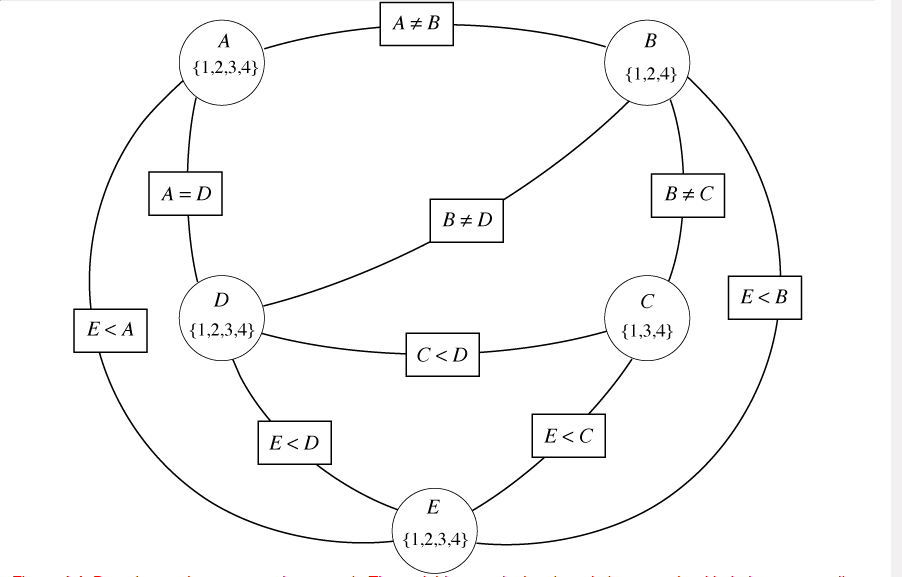
\includegraphics[width=1.0\textwidth]{images/constraint_nw.png}
  \caption[ ]{the Constraint Network for a CSP problem instance}
  \label{cs:nw}
\end{figure}

After converting the CSP into a Constraint Network a set of attributes is calculated. These attributes are to measure important features in the Constraint Network for the instance. Some of the attributes are:
\begin{itemize}
  \item \textbf{Edge density:} The number of edges in G divided by the number of pairs of distinct vertices.\\
  \item \textbf{Clustering coefficient For a vertex $v$ : } the set of neighbours of $v$ is $n(v)$. The edge density among the vertices $n(v)$ is calculated. The clustering coefficient is the mean average of this local edge density for all v \cite{f:feat}.\\
  \item \textbf{Normalised degree:} The normalised degree of a vertex is its degree divided by $|V|$. The minimum, maximum, mean and median normalised degree are used.\\
  \item \textbf{Variable domains:} The quartiles and the mean value over the domains of all
  variables.\\
  \item \textbf{Constraint arity:} The quartiles and the mean of the arity of all constraints
  (the number of variables constrained by it), normalised by the number of
  constraints.\\
\end{itemize}

These attributes along with others \cite{ml:csd} are calculated as numerical values. The numerical values are then applied to the classifier as a training data instance. The goal was to create a large set of the attributes to cover as much of the important factors as possibles. The more important the factor is the more that it affects the performance of different implementations \cite{ml:csd}. However, computing this large set of attributes required a significant amount of time that can usually reach a penalty of 27s per instance. And that time is added to the penalty of the solver itself which on average was only 0.2s per instance. And so, this makes the classifier slower than the default implementation \cite{ml:csd}. After considering this problem, The number of computed features was reduced and this lead to a significant improvement with an average of 5s per instance. Figure \ref{perf:speedup} shows the speedup achieved by the meta-classifier after computing the cheap set of features instead of computing all of them.
\\
\begin{figure}[h!]
  \vspace{1 cm}
  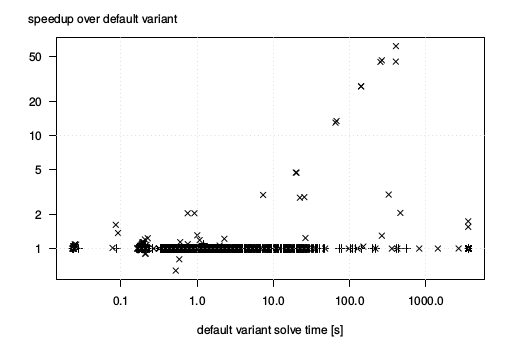
\includegraphics[width=1.0\textwidth]{images/speedup.png}
  \caption[ ]{Speedup achieved by the meta-classifier using the set of cheaply-computable
features.}
  \label{perf:speedup}
\end{figure}

The classifier was trained on 277 benchmark instances from 14 different problem classes chosen to include as many instances as possible. However, there was an important observation and that is due to the variety of the problem classes the classifier could be trained wrongly on them. But the goal here was not to train the classifier on as many different classes as possible, instead the goal was to classify the important problem classes correctly. So, in order to overcome this problem it was decided to ignore the classic Machine Learning performance measures. Measuring the performance was done in terms of the misclassification penalty, which as defined in \cite{ml:csd}, is the additional amount of CPU time required by the classifier when not choosing the fastest solver. In order to make sure that the classifier is trained correctly on the important classes of problems, each instance appeared in the training data set according to the formula $1 + log_{2}(cost)$. This formula indicates that the higher the cost of the instance, the more important it's, so it should appear in the training data set more often.
\\\\
Finally, to make sure that the classifier is as generalized as possible, $3$-\textit{fold} cross validation was used. Generally, The way $n$-\textit{fold} cross validation works is by dividing the data set into equal sized $n$ sets, then one of the n sets is used for testing and the other $n-1$ are used for training. The process is repeated until each of the n sets are used once for testing. Using stratified cross-validation will ensure that the ratio of the classification categories is roughly equal. In other words, if 50\% of the whole problem instances set were solved faster using the naive implementation, then the same ratio will be in a subset of the problem instances as well.

\clearpage
%
\section{Results}
%
In this section, we describe the speedup in performance achieved by the meta-classifier. First, the data set used for the testing consisted of 1036 benchmark instances. This set consisted of 2 problem classes different from  the ones used in the set for training the classifier. This is due to the fact that the lower the number of different problem classes the more unsuitable it's for training \cite{ml:csd}.
\\\\
The results are illustrated in the table in Figure \ref{fig:results}. The overall performance of the meta-classifier is compared with the best possible classifier and the worst one along with other classifiers such as the random decision classifier and the default decision classifier. As we can see from the table, the meta-classifier outperforms the default choice classifier, which always makes the default decision.
\\\\
Also it was observed that the set of misclassified instances for each classifier is different. In other words, the classifiers seems to complement each other. This is also shown in the table illustrated in Figure \ref{fig2:results} which provides further evidence for the fact that the performance of the meta-classifier does not suffer even if a large number of the classifiers that it combines perform badly individually. The individual best and worst classifiers vary not only with the data set, but also with the set of features used. Which indicates that the best classifier can't simply be chosen to be the idle one\cite{ml:csd}.

\clearpage
\begin{figure}[h!]
  \vspace{1 cm}
  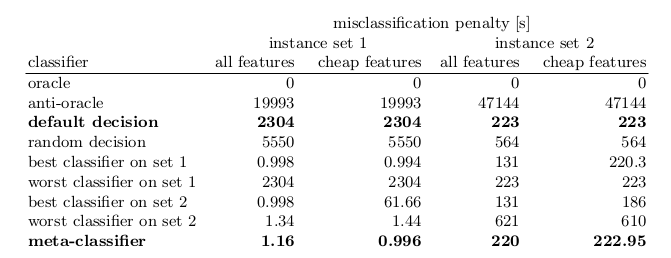
\includegraphics[width=1.0\textwidth]{images/results.png}
  \caption[ ]{Summary of classifier performance on both sets of benchmarks in terms of
total misclassification penalty in seconds.}
  \label{fig:results}
\end{figure}

\begin{figure}[h!]
  \vspace{1 cm}
  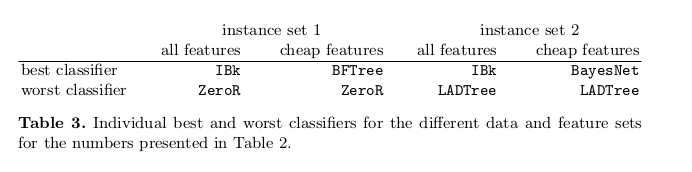
\includegraphics[width=1.0\textwidth]{images/results2.png}
  \caption[ ]{Individual best and worst classifiers for the different data and feature sets.}
  \label{fig2:results}
\end{figure}

%
\clearpage
\section{Conclusion}
%
As we have seen, Machine Learning can be applied successfully in the field of Algorithm Selection for modeling and training a classifier that is able to solve complex problems in constraints programming. We have shown how the training should be done by illustrating the modeling of the problem instance and the computing the features to be able to train the classifier.
\\\\
But in order to achieve good results. We discussed many important factors that has to be considered. Such as, computing a relatively small amount of features to avoid high penalty, caused by calculating expensive features, and at the same time making sure that the right features are calculated to cover a wide range of possible factors due to the fact that similar instances are likely to behave similarly.
\\\\
We also discussed the idea of using the common technique of duplicating the instances that was used for training.
This was done in order to push the classifiers towards learning more about the high cost instances, and to make sure that the important instances appear in the data more times than less important ones. Considering this factor affected the performance positively and reduced the misclassification penalty.
\\\\
The performance of the meta-classifier have shown an overall significant improvement over the default choice, and is able to make the correct decisions that will achieve better performance results and less penalty than using a default choice model designed by a human. The meta-classifier also as shown, is almost as good as the best classifier and much better than the worst classifier. We can conclude that with these results we have a strong evidence for the general applicability of a set of classifiers learned on a training set to sets of new, unknown instances\cite{ml:csd}.

\clearpage
%
% ---- Bibliography ----
%
\begin{thebibliography}{5}
%

\bibitem {ml:csd}
Ian P. Gent, Lars Kotthoff, Ian Miguel, Peter Nightingale:
Machine learning for constraint solver design -- {A} case study for the alldifferent constraint,
CoRR, 1008.4326 (2010)

\bibitem {gac:alldiff}
Gent, Ian P. and Miguel, Ian and Nightingale, Peter:
Generalised Arc Consistency for the AllDifferent Constraint: An Empirical Survey,
Artif. Intell. , 1973--2000, (2008)

\bibitem {f:feat}
Watts, D., Strogatz, S.:
Collective dynamics of ‘small-world’ networks. Nature 393,
440–442 (1998)

\end{thebibliography}
% \clearpage
% \addtocmark[2]{Author Index} % additional numbered TOC entry
% \renewcommand{\indexname}{Author Index}
% \printindex
% \clearpage
% \addtocmark[2]{Subject Index} % additional numbered TOC entry
% \markboth{Subject Index}{Subject Index}
% \renewcommand{\indexname}{Subject Index}
% \input{subjidx.ind}
\end{document}
